\chapter{Design}
\label{ch:design}
The design of the components used for making a robot which will be able to fulfill the requirements in section \ref{ch:Requirements for the turtlebot}, is described in this chapter.

%
% 
% DETECTION
%
%

\section{Detection} \label{ch:designDetection}
The Turtlebot is using The ASUS Xtion PRO LIVE as its vision. Xtion PRO LIVE has two microphones on each side, see figure \ref{fig:asusCamera}.\\

Nr. 1: The Xtion PRO LIVE has an RGB camera with a resolution of 640px x 480px at 30 fps, see figure \ref{fig:asusCamera}.\\ 
Nr. 2 and 4: Has a field of view distance ranging from 0.85 m up to 3.5 m and have a field of vision of 58${^\circ}$ horizontal, 45${^\circ}$ vertical and 70${^\circ}$ diagonal.
Nr. 3: Is an IR camera which has a resolution of 640px $\cdot$ 480px at 30 fps or 320px $\cdot$ 240px at 60 fps, the IR camera captures the IR projection see figure \ref{fig:asusCamera}.\\
This camera is best for indoor use \ref{ch:CameraRGB}.
\begin{figure}[h!]
    \centering
    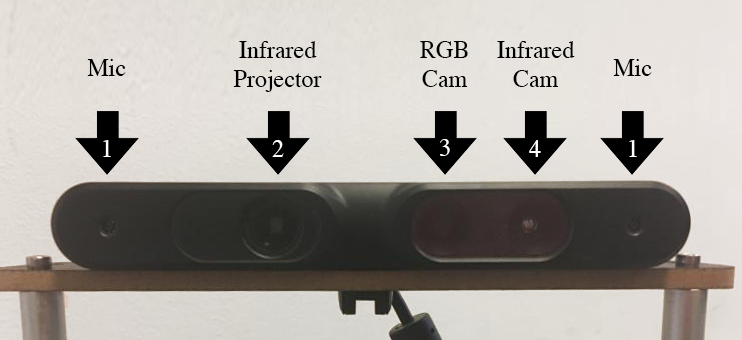
\includegraphics[width=.7\textwidth]{figures/camera02.png}
    \caption{ASUS Xtion PRO LIVE} 
    \label{fig:asusCamera} 
\end{figure}
\newpage

%bumber sensor

%
%
% PATH-PLANNING
%
%

\section{Path-planning} \label{ch:designPathplanning}
For doing path-planning, the robot is using the program Rviz, an algorithm called \textit{Frontier\_exploration} and a concept called SLAM. These are explained in this section.

\subsection{Rviz}
Rviz is a program used by ROS to provide 3D images and point clouds from data given by the robots sensors. Rviz lets the user spectate the robot in different ways. The input the robot gets from cameras and sensors is numbers and coordinates. Rviz converts these numbers into 3D objects which represents these objects \cite{interactiveMarkers}.

\subsection{Frontier\_exploration}
Frontier\_Exploration package will be used as an algorithm for the robot to navigate through a perceived environment.\\
The package provides a costmap\_2D, client/server nodes and Layer BoundedExplorerLayer. The BoundedExplorerLayer can be used for many complex explorations, functioning by two services.\\
Updatepolygonfrontier, this is where the input is telling the robot which area to scan. The service GetNextFrontier, will wait for user input and then run the first service again.\\
The robot in this project has no global map, which means the robot should be able to create a map on its own. This can be done autonomously by publishing a starting point, it will then determine its own path and act accordingly. Furthermore, it will still be able to allow user input, such as a published polygons \cite{ROSexploration}.\\
For creating a map in an unknown environment, this has been chosen.

\subsection{SLAM}
SLAM is not a specific algorithm, but a concept where there are many different approaches. That is why there are different solutions for SLAM. Some are made for indoor use, and others for outdoor use.\\
SLAM is using a mapping package called \textit{gmapping} in ROS. The gmapping package in ROS is called \textit{slam\_gmapping}. This package uses data collected from lasers and the robots position to create a 2D map.\\ %Furthermore, slam\_gmapping creates a 2D map in Rviz with lasers and position data collected by the robot.\\
When the robot starts mapping, the localization system AMCL helps the robot to move safely from one location to another.
Information from sensors, such as odometry and gyroscope, is collected when mapping. \\
By comparing data from sensors to the known map, it measures how far it has moved, furthermore it looks at the surrounding area to check its new relative position.\\The robot visualizes a map to find a trajectory to move forward. The localization system, AMCL, working-process is described in figure \ref{fig:amcl}.
\begin{figure}
    \centering
    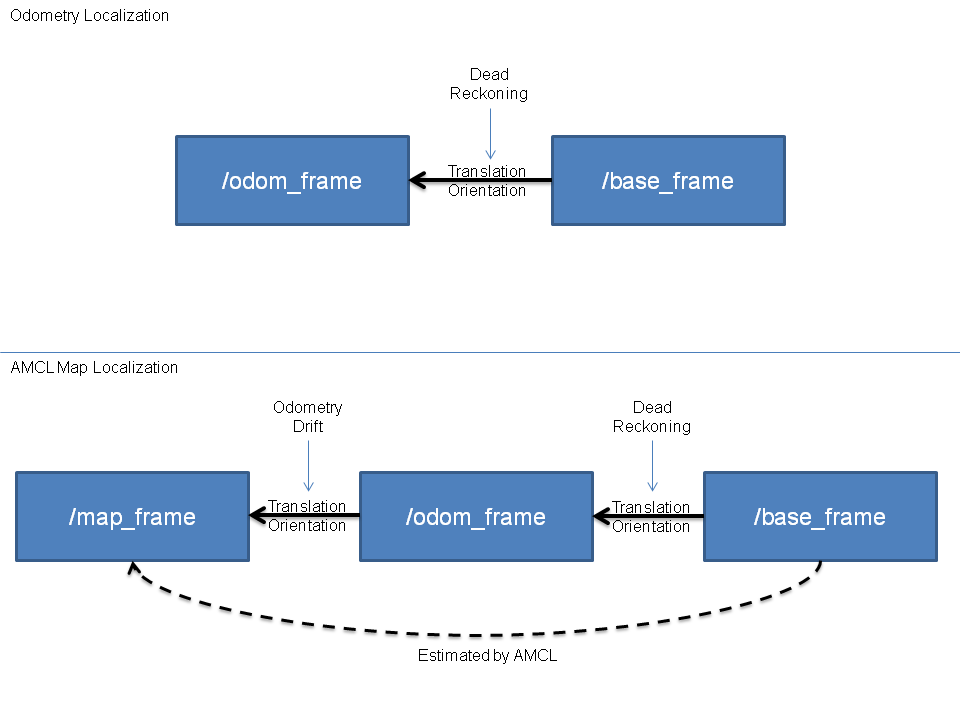
\includegraphics[width=.7\textwidth]{figures/AMCL.png}
    \caption{AMCL working process\cite{AMCL}} 
    \label{fig:amcl} 
\end{figure}
 During operation, AMCL estimates the transformation of the base frame in respect to the global frame. But it only publishes the transformation between the global frame and the odometry frame\cite{AMCL}.

%
%
% MOVEMENT
%
%

\section{Movement}\label{ch:designMovement}
To move the turtlebot manually, the user can use the terminal to deliver velocity commands to the robot. When using frontier exploration node, the user appoints an area to be searched in Rviz. The frontier node calculates a small path to be explored, this gets translated into velocity commands by the move\_base node. The velocity commands gets converted into a PWM signal to the motor driver for the turtlebot.

\subsection{Manual navigation}
Before it is possible to send any data to the turtlebot, a node has to be built. In this node a publisher has to be declared, to send a message on a topic. In this node topic is /move\_base\_simple/goal and the message types it send is a geometry\_msgs::PoseStamped, see figure \ref{fig:nodehandle}.
\begin{figure}[h]
    \centering
    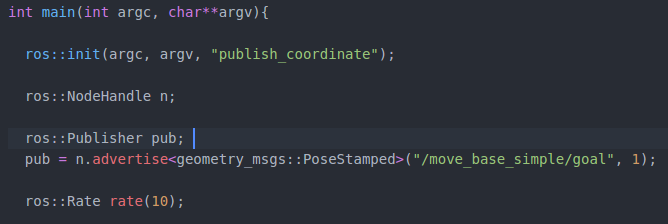
\includegraphics[width=.8\textwidth]{figures/initByC.png}
    \caption{Initializing nodehandel} 
    \label{fig:nodehandle} 
\end{figure}


The geometry\_msgs::PoseStamped contains different members, it has a header member and a pose member. Inside the Pose member there are more member positions and orientations, in the member position a x, y and z coordinate can be stated for the turtlebot to move to, but there are no need to state the z coordinate because the turtlebot only works on a bi-dimension plane.\\ 
The heading is set by the z orientation member, see figure \ref{fig:msg}.\\
\begin{figure}[h!]
    \centering
    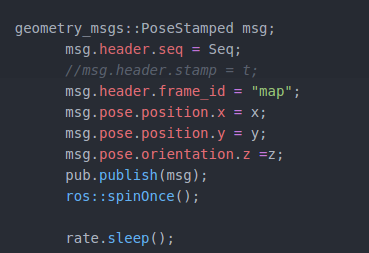
\includegraphics[width=.5\textwidth]{figures/msgbyc.png}
    \caption{Publishing a messages.} 
    \label{fig:msg} 
\end{figure}
%\newpage
One thing to remember is that orientation is always relative to the turtlebot, meaning that the x axis is directly in the front to the back of the turtlebot, and the y axis is going through the sides of the turtlebot.\\
When the user has entered some coordinates, the message get published with the information which the user entered. The /move\_base\ is subscribing to the topic /move\_base\_simple/goal. The /move\_base\ will then publish to frontier\_exploration node, which will then make a path based on the information which is already on the map.
